% This is based on "sig-alternate.tex" V1.9 April 2009
% This file should be compiled with V2.4 of "sig-alternate.cls" April 2009
%
\documentclass{report}

\usepackage[english]{babel}
\usepackage{graphicx}
\usepackage{tabularx}
\usepackage{subfigure}
\usepackage{enumitem}
\usepackage{url}
\usepackage{float}

\usepackage{color}
\definecolor{orange}{rgb}{1,0.5,0}
\definecolor{lightgray}{rgb}{.9,.9,.9}
\definecolor{java_keyword}{rgb}{0.37, 0.08, 0.25}
\definecolor{java_string}{rgb}{0.06, 0.10, 0.98}
\definecolor{java_comment}{rgb}{0.12, 0.38, 0.18}
\definecolor{java_doc}{rgb}{0.25,0.35,0.75}

% code listings

\usepackage{listings}
\lstloadlanguages{Java}
\lstset{
	language=Java,
	basicstyle=\scriptsize\ttfamily,
	backgroundcolor=\color{lightgray},
	keywordstyle=\color{java_keyword}\bfseries,
	stringstyle=\color{java_string},
	commentstyle=\color{java_comment},
	morecomment=[s][\color{java_doc}]{/**}{*/},
	tabsize=2,
	showtabs=false,
	extendedchars=true,
	showstringspaces=false,
	showspaces=false,
	breaklines=true,
	numbers=left,
	numberstyle=\tiny,
	numbersep=6pt,
	xleftmargin=3pt,
	xrightmargin=3pt,
	framexleftmargin=3pt,
	framexrightmargin=3pt,
	captionpos=b
}

% Disable single lines at the start of a paragraph (Schusterjungen)

\clubpenalty = 10000

% Disable single lines at the end of a paragraph (Hurenkinder)

\widowpenalty = 10000
\displaywidowpenalty = 10000

% allows for colored, easy-to-find todos

\newcommand{\todo}[1]{\textsf{\textbf{\textcolor{orange}{[[#1]]}}}}

% consistent references: use these instead of \label and \ref

\newcommand{\lsec}[1]{\label{sec:#1}}
\newcommand{\lssec}[1]{\label{ssec:#1}}
\newcommand{\lfig}[1]{\label{fig:#1}}
\newcommand{\ltab}[1]{\label{tab:#1}}
\newcommand{\rsec}[1]{Section~\ref{sec:#1}}
\newcommand{\rssec}[1]{Section~\ref{ssec:#1}}
\newcommand{\rfig}[1]{Figure~\ref{fig:#1}}
\newcommand{\rtab}[1]{Table~\ref{tab:#1}}
\newcommand{\rlst}[1]{Listing~\ref{#1}}

% General information

\title{Kompose\\
\normalsize{A Distributed Playlist for Android}}
\subtitle{subtitle}

% Use the \alignauthor commands to handle the names
% and affiliations for an 'aesthetic maximum' of six authors.

\numberofauthors{2} %  in this sample file, there are a *total*
% of EIGHT authors. SIX appear on the 'first-page' (for formatting
% reasons) and the remaining two appear in the \additionalauthors section.
%
\author{
	\alignauthor\normalsize{Mark Arnold, Dino Bollinger, Tobias Brodmann}\\
	\affaddr{\normalsize{15-917-701, 14-923-676, 15-934-565}}\\
	\email{\normalsize{arnomark@student.ethz.ch, bdino@student.ethz.ch, brotobia@student.ethz.ch}}
\alignauthor \normalsize{Lino Lendi, Florian Moser, Lukas Tobler}\\
	\affaddr{\normalsize{11-714-383, 15-930-704, 14-942-007}}\\
	\email{\normalsize{llendi@student.ethz.ch, moserfl@studen.ethz.ch, lutobler@student.ethz.ch}}
}

\begin{document}

\maketitle

\begin{abstract}
\emph{Kompose} is an Android application that aims to allow multiple independent participants to form 
a local party through which they share a music playlist and request songs to be played at social events.
The songs will be downloaded from Youtube, and each participant will be able to share, synchronize and 
vote on what song they want to be played next in a fully distributed fashion. One device will act as the host 
which controls the playback of the queue, while the order of the songs will be agreed upon by all clients.

\end{abstract}
%
\section{Introduction}
At social events, such as clubs or parties, we often face the problem of deciding which person should be
in charge of the music being played. From our experience, many people often disagree with a particular 
DJs taste in music, and are subsequently dissatisfied with the chosen playlist. And even if the DJ only takes
suggestions from the participants themselves, there may often be fringe tastes that are only enjoyed by a 
small minority while others are left completely alienated. The DJ may also be overwhelmed by requests, and
would benefit greatly from a simple way for people to keep track of what has already been requested.\\\\
%
\emph{Kompose} solves this problem by creating a distributed playlist that anyone
can add songs to. 
One device will start a session (the \emph{host}, usually connected
to a stereo), and other devices on the local network can join in and start
adding songs to the queue. Apart from choosing the name for the party and 
being responsible for the playback, in terms of voting, the host will have 
the same rights as the other clients in the system.
Clients can \emph{downvote} a specific song, and once a majority of clients 
downvoted a song, it will be removed from the queue.  
Past sessions will be kept, so the users can review playlists at a later date.\\\\
%
The primary source of music will be YouTube. Clients send their song request 
in the form of a youtube URL to the host. The host will then download and cache the
audio from YouTube one song ahead of time to allow continuous playback. This will allow
us to keep a large playlist without having to store all songs at once.\\\\
%
The challenges in this project are as follows: 
\begin{itemize}
	\item Automatically announcing and finding other \emph{Kompose} services on the network.
	\item Synchronizing the playlist state to all devices.
	\item Keeping track of all clients that are still alive to allow the majority based voting.
	\item Adding new songs to the playlist, and voting on skipping songs should be fair for all clients.
	\item Finally, a protocol that supports all these features must be devised.
\end{itemize}

\section{System Overview}
\subsection{Client/Server architecture}

Each device running the app can choose to become host, at which point it will
act as the server in our system. All communication is done over these hosts, 
i.e. there is no peer-to-peer communication between other clients.
To support this, we will define a custom application-level communication protocol 
and will provide at least the following functionality:
\begin{itemize}
\item Sending client registration and deregistration messages
\item Sending song requests and skip messages from clients to server.
\item Aliveness messages for clients, to determine whether a participant and/or host is still active
\item Sending playlist state (including all songs in the play queue, at the received downvotes for each of the songs) to the clients.
\item Various error messages
\end{itemize}
%
The messages of this protocol will be transported over TCP in the form of JSON.\\\\
%
Both client and server listen on the network for messages,
the host for requests from the clients, and the clients for state updates
from the host. To avoid manual IP/port configuration, \emph{Network Service Discovery}
\cite{nsd} is used. This gives the clients the hosts' IP and port,
to which they can send a \emph{register} messgage containing the IP and port they
will be listening on for state updates. \\\\
%
Once a client is connected to the host, he can start sending song request and vote messages.
Song requests will cause the corresponding song to be added to the playlist unless
it already exists in the queue. Vote-Skip messages help make the participants reach
consensus over which songs they want to play. Once a song receives skip requests
from a majority of the clients, the song will be removed from the playlist.\\\\ 
%
To add some resilience against clients dropping off the network, clients periodically 
send a keep-alive message to their host every few seconds, and vice-versa.
If a client becomes unresponsive, he will be dropped from the party and the maximum number of votes
necessary to remove a song from the playlist will decrease accordingly. This serves to
ensure that the voting system does not become unresponsive should a majority of clients crash.\\\\
%
In the case that the host crashes or become otherwise unreachable, then the party will be 
disolved gracefully. If time allows, we may also explore options to dynamically switch 
the host to one of the party members.
%

\subsection{User interface}
The \emph{Kompose} app will consist of at least 6 different activities in total, 
each serving a unique purpose, as well as several popup windows which will offer 
further options to the user. \\\\
%
Figure 1 shows a mockup of this user interface design. The start screen
(top center) allows the user to either join a pre-existing party, or 
create an entirely new one. When creating a new party, the host chooses 
a new name which will be visible for all clients in the LAN, and then
proceeds to the playlist itself. Here he will continuously listen for new
connections and send out new discovery messages in periodic intervals. \\\\
%
When choosing to join a party, the clients will be sent to a different
activity that displays a list of all currently available parties.
If an announcement from a host is received, the party name shows up in 
this list and can be joined. Once the choice is made, the client is sent
to the main playlist interface. \\\\
%
In addition to these two options, there is also a third which will send 
the user to the history of all playlists of previous sessions.
Once a party is closed, the current playlist is saved on local storage,
so that they can later be viewed by the user. This feature is non-critical 
for the proper function of the app, but it is nonetheless a welcome service
for the user. \\\\
%
The main playlist interface will display a list of all items currently in 
the play queue. This queue is displayed in the order in which songs will be 
played by the host, from first to last in line. Each list element will display 
at least the title of the file, as well as the URL from where the audio has 
been retrieved. Finally, each list item includes a designated downvote button,
which serves to cause unpopular songs to be removed from the queue. As soon as 
a majority of the clients deem a song bad, it will no longer appear in the queue. \\\\
%
The host will additionally have a play/pause button in the action bar.

\subsection{YouTube file downloads}
Songs are fetched from YouTube by the host only, using a library \cite{youtubeExtractor}
to extract the URL for the audio file. Songs in the play queue are pre-fetched
one song ahead of time to guarantee continuous playback. The number of items that 
are cached can be configured in the settings. This is of course handled asynchronously in
the background.

\section{Requirements}

	\paragraph{Discovery service}
	We will use the Android Network Service Discovery API \cite{nsd} as provided by android itself
	to enable the client-server discovery in the network
	
	\paragraph{YouTube Downloads}
	We will enable users to put videos from youtube inside the play queue. To fetch the audio
	URLs from those videos we will rely on a library called android-youtubeExtractor \cite{youtubeExtractor}

\section{Work Packages}
To work efficiently, and enable group members to work in their area of expertise
we will divide the group coarsely into a technical and a design team.
With this in mind, our work packages are split by technical and design aspects, but 
the designers and the developers will stay in close contact throughout the whole process.

\paragraph{WP1: Protocol specification}
The technical group will firstly define a protocol to support all required functionalities.
Much time will be spent on this. A well defined protocol will ease up development and
help with further updates of the application. The target of this work package is the
definition of a small but extensible protocol.

\paragraph{WP2: Client/Server implementation}
This work package includes the implementation of the defined protocol in \emph{WP1}
with all functionality as defined in this document by the technical team. The target of this 
work package is a fully functional prototype.

\paragraph{WP3: User interface design}
Parallel to WP1 and WP2 the design team will work on the interface look \& feel. 
Besides the design, the group will focus on usability aspects, and will be in close
contact to the development group. The target of the work package is a consistent 
design of the various pages which fits to its target user group.

\paragraph{WP4: UI implementation}
After finishing the design it will be implemented using the prototype from \emph{WP3}.
Target of this work package is the nearly finished application.

\paragraph{WP5: Testing \& polish}
For this last work package the design and technical team will work together
on finalizing the functions and design of the application. Inputs from people from outside 
the projects will also be evaluated. Target of this work package is to polish the design,
and confirm that all functionality works as intended and as advertised in the UI.

\section{Milestones}

\subsection{Milestone technical}
The technical milestone will include both \emph{WP1} and \emph{WP2} and will be done by our technical team,
consisting of the members lutobler, brotobia and bdino.
They have already started with their work packages, and will finish the milestone by 25.11.17 at latest.

\subsection{Milestone design}
The design milestone will include both \emph{WP3} and \emph{WP4} and will be completed by our design team, 
consisting of moserfl, llendi and arnomark. While \emph{WP3} is already in progress, \emph{WP4} will start
after \emph{Milestone technical} is completed. Both work packages will be done by 02.12.17

\subsection{Milestone testing}
After the completion of the first two milestones, all team members will come together to test and polish the application
as described in \emph{WP5}. The testing phase will finish at 14.12.17 at latest, shortly after the application and 
all additional material will be submitted. This will respect all of the fixed deadlines:

\begin{itemize}
    \item {\bf 15.12.2017:} Presentation/Logo deadline
    \item {\bf 17.12.2017:} Code deadline
    \item {\bf 18.12.2017:} Presentation and demo session
\end{itemize}

% The following two commands are all you need in the
% initial runs of your .tex file to
% produce the bibliography for the citations in your paper.
\bibliographystyle{abbrv}
\bibliography{report}  % .bib is the name of the Bibliography in this case
% You must have a proper ".bib" file

%\balancecolumns % GM June 2007
\begin{figure*}
    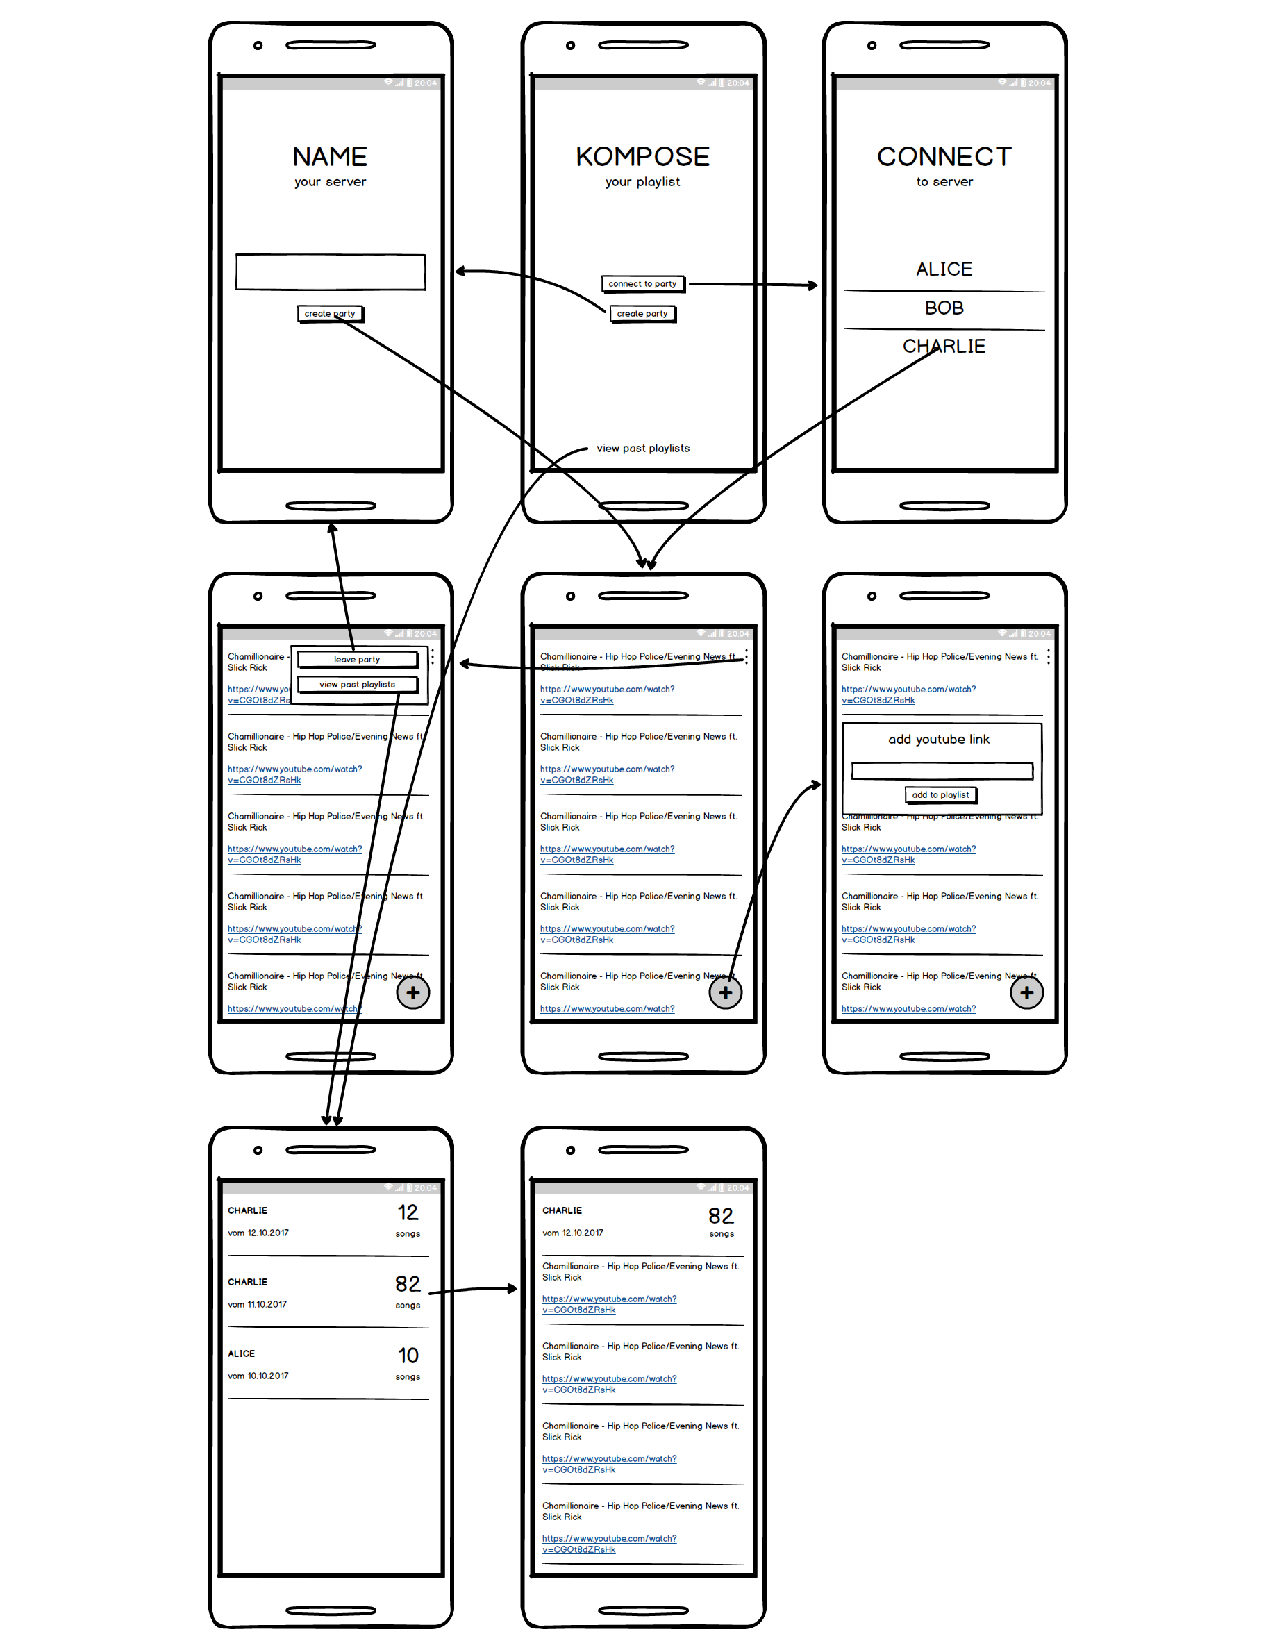
\includegraphics[width=\textwidth]{../design/mockups.pdf}
    \caption{User interface mockup (created with \cite{balsamiq})}
\end{figure*}

\end{document}
